Given, 
\begin{align}
	x^2 + 2y - 3 &= 0 \label{eq:solutions/1/22/eq:eq1}
\end{align}
From \eqref{eq:solutions/1/22/eq:eq1}, 
\begin{align} 
    \vec{V} &= \myvec{1 & 0 \\ 0 & 0} \label{eq:solutions/1/22/eq:eq2} \\
    \vec{u} &= \myvec{0 \\ 1} \\
    f &= -3
\end{align}
From \eqref{eq:solutions/1/22/eq:eq2},
\begin{align}
    \mydet{V} = \mydet{1 & 0 \\ 0 & 0} = 0 \label{eq:solutions/1/22/eq:eq3}
\end{align}
Now \eqref{eq:solutions/1/22/eq:eq3} implies that the curve is a parabola. We can find the Eigen values corresponding to the $\vec{V}$,
\begin{align}
    \mydet{V-\lambda I} &= 0 \nonumber \\
    \mydet{1-\lambda & 0 \\ 0 & -\lambda} &= 0 \nonumber \\
    \implies \lambda &= 0,1 \label{eq:solutions/1/22/eq:eq4}
\end{align}
Calculating the Eigen Vectors corresponding to $\lambda=0,1$ respectively,
\begin{align}
    \vec{V}\vec{x} = \lambda\vec{x} \nonumber 
\end{align}
\begin{align}
    \myvec{1 & 0 \\ 0 & 0}\vec{x} = 0;\implies \vec{p}_1 = \myvec{0 \\ 1} \label{eq:solutions/1/22/eq:eq5} \\
    \myvec{0 & 0 \\ 0 & -1}\vec{x} = 0;\implies \vec{p}_2 = \myvec{1 \\ 0} \label{eq:solutions/1/22/eq:eq6}
\end{align}
By Eigen decomposition on $\vec{V}$,
\begin{align}
    \vec{V} = \vec{P}\vec{D}\vec{P}^T \nonumber \\
    where, \vec{P} = \myvec{\vec{p}_1 & \vec{p}_2} = \myvec{0 & 1 \\ 1 & 0} \label{eq:solutions/1/22/eq:eq7} \\
    \vec{D} = \myvec{\lambda_1 & 0 \\ 0 & \lambda_2} = \myvec{0 & 0 \\ 0 & 1} \label{eq:solutions/1/22/eq:eq8}
\end{align}
To find the vertex of the parabola,
\begin{align}
    \myvec{\vec{u}^T+\eta \vec{p}_1^T \\ \vec{V}}\vec{c} = \myvec{-f \\ \eta \vec{p}_1-\vec{u}} \label{eq:solutions/1/22/eq:eq9} \\
    where, \eta = \vec{u}^T\vec{p}_1 = 1 \label{eq:solutions/1/22/eq:eq10}
\end{align}
Substituting values from \eqref{eq:solutions/1/22/eq:eq2}, \eqref{eq:solutions/1/22/eq:eq5} and \eqref{eq:solutions/1/22/eq:eq10} in \eqref{eq:solutions/1/22/eq:eq9}, 
\begin{align}
    \myvec{0 & 2 \\ 1 & 0 \\ 0 & 0}\vec{c}=\myvec{3 \\ 0 \\ 0} \label{eq:solutions/1/22/eq:eq11}
\end{align}
Removing last row and representing \eqref{eq:solutions/1/22/eq:eq11} as augmented matrix and then converting the matrix to echelon form,
\begin{align}
    \myvec{0 & 2 & 3 \\ 1 & 0 & 0} \xleftrightarrow[]{R_1\leftrightarrow R_2} \myvec{1 & 0 & 0 \\ 0 & -2 & -3}\\
    \myvec{1 & 0 & 0 \\ 0 & -2 & -3} \xleftrightarrow[]{R_2\leftarrow -\frac{R_2}{2}} \myvec{1 & 0 & 0 \\ 0 & 1 & \frac{3}{2}}\label{eq:solutions/1/22/eq:eq12}
\end{align}
From \eqref{eq:solutions/1/22/eq:eq12} it can be observed that,
\begin{align}
    \vec{c} = \myvec{0 \\ \frac{3}{2}} \label{eq:solutions/1/22/eq:eq13}
\end{align}
Now to evaluate the direction vector $\vec{m}$,
\begin{align}
    \vec{m}^T(\vec{V}\vec{q} + \vec{u}) &= 0 \\
    \vec{m}^T\myvec{\myvec{1 & 0 \\ 0 & 0}\myvec{1 \\ 1} +\myvec{0 \\ 1}} &= 0 \\
    \vec{m}^T\myvec{\myvec{1 \\ 0} +\myvec{0 \\ 1}} &= 0 \\
    \vec{m}^T\myvec{1 \\ 1} &= 0 \\
    \implies \vec{m} &= \myvec{1 \\ -1} \label{eq:solutions/1/22/eq:eq14}
\end{align}
Now to obtain the equation of normal using,
\begin{align}
    \vec{m}^T(\vec{x} - \vec{q}) &= 0 \\
    \myvec{1 & -1}\myvec{\vec{x} - \myvec{1 \\ 1}} &= 0 \\
    \myvec{1 & -1}\vec{x} &= 0 
\end{align}
\begin{figure}[h!]
\centering
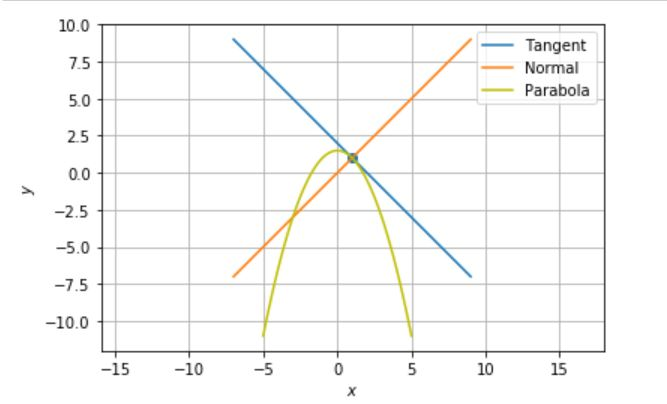
\includegraphics[width=\columnwidth]{./solutions/1/22/Plot.JPG}
\caption{{Parabola showing tangent perpendicular to the normal}}
\label{eq:solutions/1/22/myfig}
\end{figure}
